\chapter{Implementation}\label{ch:implementation}

% demonstrate feasibility
% Overview
%     programming lanagaueg, streaming frameowkr, cep engine used

% event representation
%     data strucvture, seralization format, metadata encoding
% stream processing pipeline
%     threading mode, buffering, ordering
% coordinator implementation  
%     timeout, clock management, late event handling
% reconstructuion logic
%     event sysnthesis, timestamp assignment, source attribution
% predictor implementation
%     Kalman filter stats, state vector definition, noise parameter selectionm
% confidence computation
%     prediction evaluation, numerical stability, performance considerations
% CEP
%     query examples, confidence aware predicates, compatibility
% performance considerations
%     latency, throughoutput, state size
% Limitations
%     parameter sensitivity
%     computational overhead
%     scalability constrants






    \section{Implementation}
\label{sec:implementation}

This section describes the concrete implementation of the proposed architecture, with particular emphasis on the cross-language integration between the reconstruction and event processing layers. The implementation follows the architectural design introduced in Chapter~\ref{ch:architecture} and realizes its components using a combination of Python and Java technologies.

\begin{figure}[t]
    \centering
    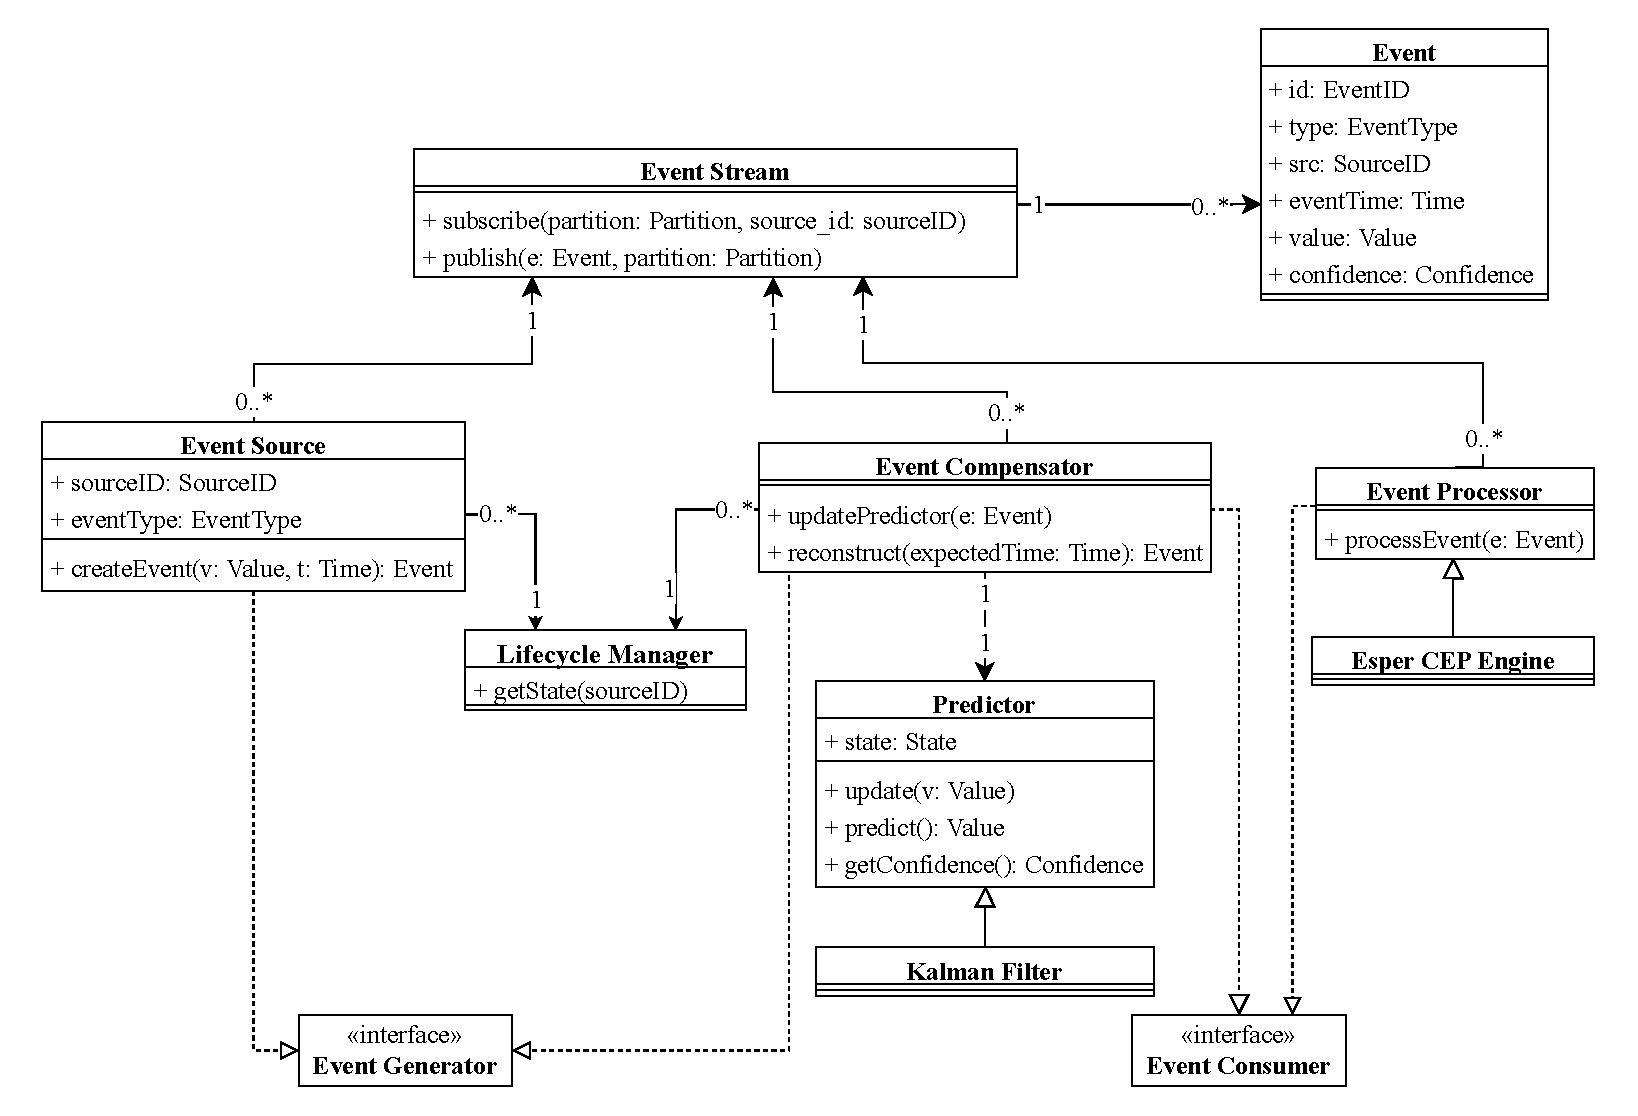
\includegraphics[width=\textwidth]{figures/Architecture/UML Model.drawio.pdf}
    \caption{UML model of the implemented system.}
    \label{fig:uml-model}
\end{figure}

\subsection{Cross-Language Architecture}

The system is implemented as a distributed, event-driven pipeline spanning two programming languages. The reconstruction and coordination components are implemented in Python~3.10, while the complex event processing (CEP) engine is implemented in Java~21 using the Esper framework.

This division reflects the differing requirements of the two subsystems. The reconstruction layer relies on numerical computation and state estimation techniques, for which Python provides mature libraries and rapid development support. In contrast, complex event processing requires efficient execution of continuous queries over high-volume event streams, an area where Java-based CEP engines such as Esper are well established.

To enable interoperability between these subsystems, all communication occurs through a shared event stream abstraction. This design allows the Python and Java components to operate independently while exchanging events using a common schema and transport mechanism.

\subsection{Event Stream and Communication Layer}

The event stream is implemented using ZeroMQ as a lightweight message bus. A server component provides the underlying publish–subscribe and push–pull socket topology, while clients connect to the server to publish and consume events. The event stream itself is implemented as a client that manages event partitions and dispatches events to registered consumers.

This separation ensures that components do not communicate with each other directly but instead interact exclusively through the event stream. As a result, additional components—such as visualization tools or alternative processing engines—can be integrated without modifying existing implementations.

To formalize interactions with the event stream, two interfaces are defined: \texttt{EventGenerator} and \texttt{EventConsumer}. Components that produce events implement the generator interface, while components that react to events implement the consumer interface. This abstraction enforces a uniform interaction pattern across the system and supports extensibility across languages.

\subsubsection{Event Representation}

Events are represented using a language-neutral schema serialized as JSON. Each event includes a unique identifier, source identifier, event timestamp, value, confidence, and status indicating whether the event is observed or reconstructed. Additional metadata fields support extensibility without modifying the core schema.

The event schema is validated at runtime to ensure that malformed events do not enter the event stream. This validation step enforces consistency across components and prevents downstream processing errors.

\subsection{Coordination and Reconstruction}

The coordinator is implemented as an event consumer that monitors the arrival of observed events and reasons about their expected timing. For each event source, it maintains a schedule derived from configuration parameters such as sampling interval and tolerance. The coordinator operates as a discrete-event scheduler over expected observation deadlines.

When an expected event does not arrive within its configured time window, the coordinator triggers reconstruction for the corresponding source. Each source is associated with a dedicated reconstructor, which maintains predictor state and performs reconstruction when notified of missing observations.

Reconstructed events are emitted back into the event stream with associated confidence values, ensuring that downstream components observe a unified stream containing both observed and reconstructed data.

\subsection{Predictive Model}

The predictor used in this implementation is a Kalman filter. Kalman filters are well suited to event-driven state estimation due to their recursive update structure and explicit representation of uncertainty through covariance. Observed events are used to update the filter state, while missing observations are handled by state extrapolation.

The predictor exposes both estimated values and confidence measures, which are incorporated into reconstructed events. The predictor implementation is modular, allowing alternative estimation techniques to be substituted without affecting coordination or event processing logic.

\subsection{Complex Event Processing}

The event processor is implemented in Java using the Esper CEP engine. Esper evaluates continuous queries over the event stream and supports both atomic and complex event patterns. Atomic patterns match individual events based on attribute predicates, while complex patterns are defined hierarchically using combinations of atomic and other complex patterns.

Pattern definitions are loaded from JSON and compiled into Esper’s Event Processing Language (EPL). Detected patterns are represented explicitly as pattern objects that retain confidence information and traceability to contributing events. Complex patterns aggregate confidence values from their constituent patterns according to the aggregation strategy specified in their definitions.

Detected patterns are emitted back into the event stream, enabling higher-level patterns to be defined over previously detected ones. This hierarchical approach allows complex event definitions to be built incrementally while preserving confidence propagation across pattern layers.







% Python~3.10 is used for the reconstruction layer. It provides extensive libraries for numerical computation and state-estimation methods, and its flexibility supports rapid prototyping of predictive components.

% The CEP engine is implemented in Java~21 using the Esper library. The project is built with Maven (version~3.6), which compiles and packages the engine into a self-contained executable JAR. Esper provides an efficient runtime for evaluating continuous event queries, enabling low-latency processing of both observed and reconstructed events.

% To connect the Python-based reconstruction layer with the Java-based CEP engine, the system uses lightweight message passing through ZeroMQ~\cite{zeromq_org}. This design keeps the components decoupled, allowing each subsystem to evolve, be replaced, or be scaled independently without modifying the other.


% \subsection{Libraries and Tools}
% Several libraries support the implementation:

% \begin{itemize}
%     \item \textbf{NumPy} and \textbf{pandas} for numerical computation and time-indexed event manipulation.
%     \item \textbf{SciPy} for interpolation and auxiliary statistical routines.
%     \item \textbf{FilterPy} for implementing the Kalman filter used by the predictor.
%     \item \textbf{matplotlib} for evaluation plot visualizations.
%     \item \textbf{pytest} for automated testing.
%     \item \textbf{Esper} (Java) serves as the CEP engine, executing continuous queries and time-windowed pattern detection without modification to its query model.
%     \item \textbf{ZeroMQ (pyzmq)} provides asynchronous publish–subscribe communication between components
% \end{itemize}
